\subsection{Die Konfiguration des Spawners}
\todo{Noch in Arbeit}
\todo{Deadline: 26.06.}

\begin{figure}[!hb]
	\centering
	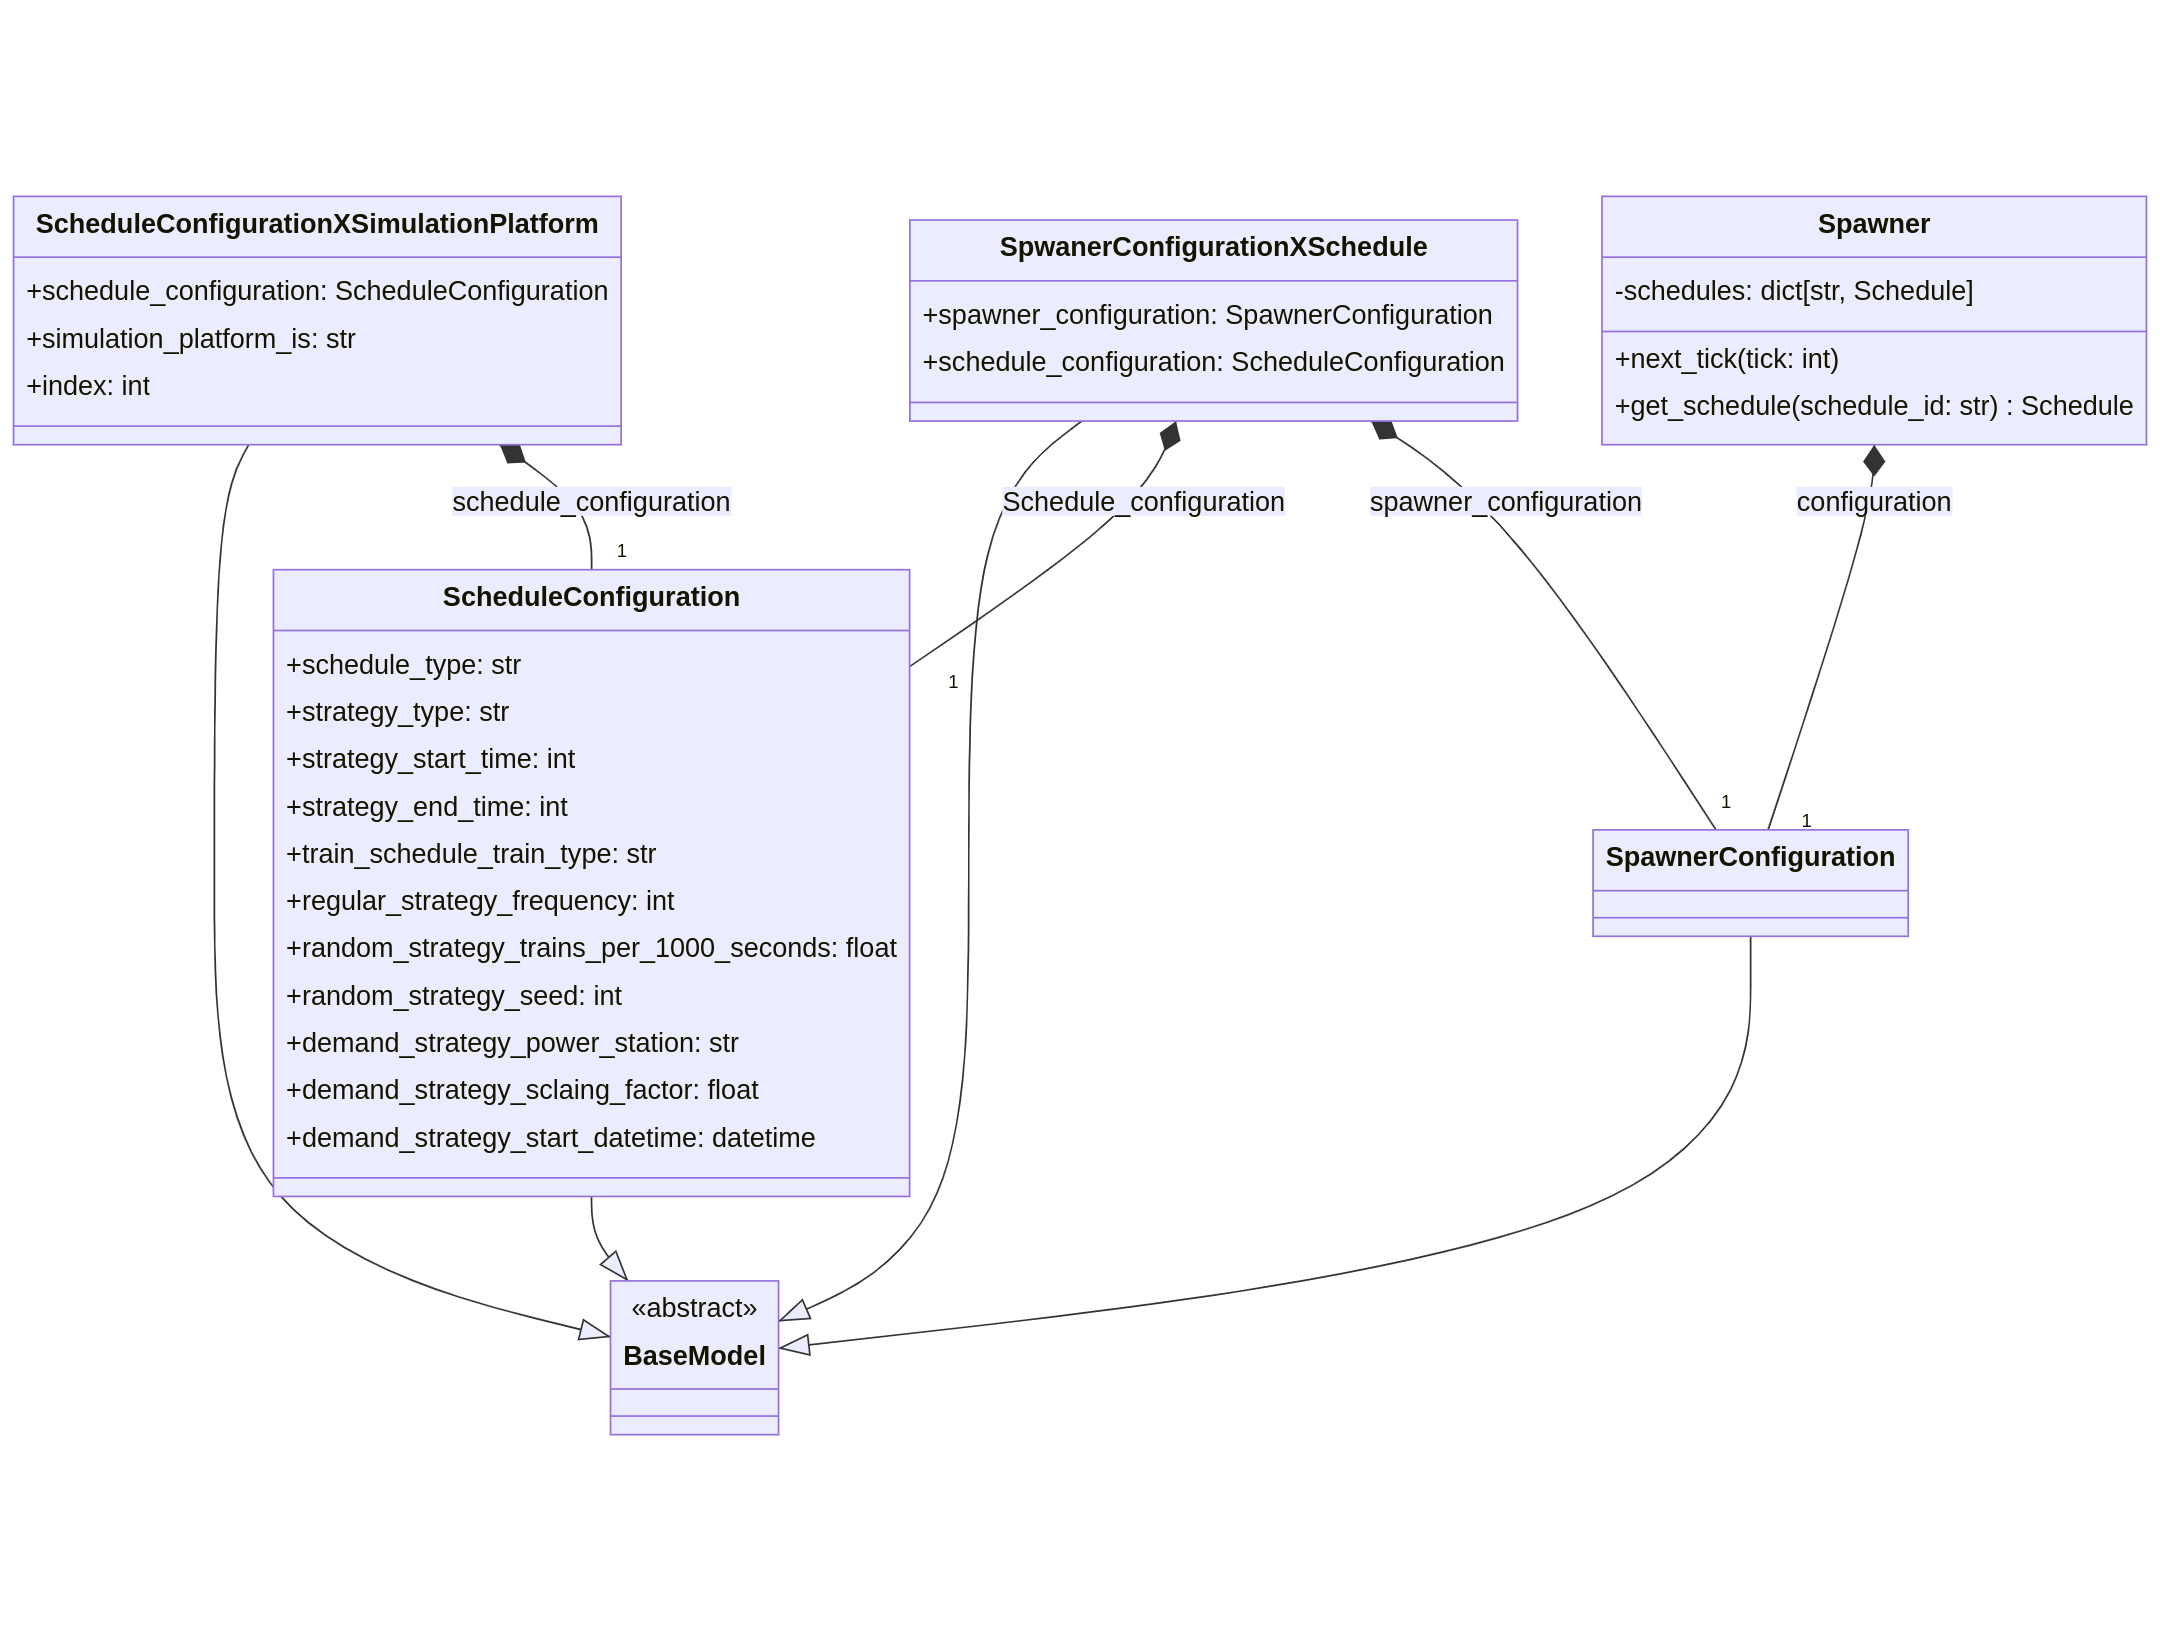
\includegraphics[width=0.75\linewidth]{images/diagrams/spawner-config-class.png}
	\caption{Klassendiagramm Spawnerkonfiguration}
	\label{fig:spawner-config-class}
\end{figure}

Der *Spawner* und insbesondere dessen *Schedules* und *ScheduleStrategies* müssen konfiguriert werden. Zum Zweck der Nachvollziehbarkeit und der Reproduzierbarkeit, müssen diese Konfigurationen persistent gespeichert werden. Dazu werden sie als Objekte in der Datenbank abgelegt.

Die initiale Idee zur Umsetzung dessen, war die konkreten *Schedules* und *ScheduleStrategies* als Spezialisierung von *BaseModel* anzulegen und somit eine Persistenz dieser Objekte in der Datenbank zu ermöglichen. Die hätte für den *Schedule* eine Vererbungshiearchie der Form *BaseModel* <- *Schedule* <- *Konkreter Schedule* zur Folge gehabt (analog für die *ScheduleStrategies*). Das von uns verwendete ORM setzt abstrakte Klassen in Form konkret existierender Datenbankrelationen um. Diese Relationen wären entsprechend stets leer. Da jedoch zur Laufzeit Variablen abstrakten Typs auf eben diese Relationen abgebildet werden, war diese Entwurfsidee keine Option für uns.

Stattdessen haben wir uns dazu entschieden, die Konfiguration von der Logik zu trennen und für die Konfiguration auf Vererbung zu verzichten. Dies löst das Problem der abstrakten Klassen mit dem ORM und ermöglicht weiterhin die Verwendung von Spezialisierung für die Funktionalität.

Die Konfiguration der *Schedules* und *ScheduleStrategies* ist nun in einer einigen Klasse, der *ScheduleConfiguration*, zusammengefasst. Dies erschien sinnvoll, da eine 1:1-Beziehung zwischen beiden Klassen besteht.

Zwischen dem *Spawner* und dem *Schedule* besteht eine m:n-Beziehung, da ein Spawner mehrere Schedules besitzen kann. Ebenso kann ein Schedule in mehreren *Spawners* Verwendung finden. Die Beziehung zwischen der *ScheduleConfiguration* und der *SpawnerConfiguration* wird daher über die Hilfsklasse *SpawnerConfigurationXSchedule* realisiert. Diese Klasse ist leer und lediglich eine technische Notwendigkeit zur Spezifikation der m:n-Beziehung für den ORM.

Ein Schedule benötigt eine Liste von Stationen, welche der Zug nacheinander ansteuern soll. Er wird an der ersten dieser Stationen erzeugt und wird an der letzten Station aus der Simulation entfernt. Diese Stationen existieren nur im Laufzeitkontext, sind also nicht in der Datenbank abgelegt. Die Klasse *ScheduleConfigurationXSimulationPlatform* repräsentiert die m:n-Beziehung zwischen einer Station und einen *Schedule*. Da m:n-Beziehungen in relationalen Datenbankmodellen ungeordnet sind, wird jedem Element dieser Beziehung ein Index zugeordnet, um eine Totalordnung über alle Elemente aufzubauen. Diese legt die Reihenfolge der Stationen fest.

Die Konstruktion der *Schedules* und *ScheduleStrategies* erfolgt durch die Factory-Methoden *strategy\_from\_schedule\_configuration* im abstrakten *Schedule* und *from\_schedule\_configuration* in den entsprechenden konkreten Strategieklassen.
